
\section{Izotermik jarayon}


\begin{enumerate}

\item Boyl-Mariott ideal gaz uchun qanday bog‘lanishni o‘rgangan?
\begin{enumerate}[label=\Alph*)]
\item $p \sim V$
\item $p \sim T$
\item $V \sim T$
\item $p \sim 1/V$
\end{enumerate}

\item Qaysi jarayonda molekulalarning o‘rtacha kinetik energiyasi o‘zgarmaydi?
\begin{enumerate}[label=\Alph*)]
\item izoxorik
\item izotermik
\item adiabatik
\item izobarik

\end{enumerate}

\item Izotermik jarayonda ...
\begin{enumerate}[label=\Alph*)]
\item $p, V$ va $T$ o‘zgaradi va tashqi muhit bilan issiqlik almashinish yuz bermaydi.
\item $V$ va $T$ o‘zgaradi, $p$ o‘zgarmaydi.
\item $p$ va $T$ o‘zgaradi, $V$ o‘zgarmaydi.
\item $P$ va $V$ o‘zgaradi, $T$ o‘zgarmaydi.
\end{enumerate}

\item Izotermik jarayon deb qanday jarayonga aytiladi?
\begin{enumerate}[label=\Alph*)]
\item doimiy issiqlik sig‘imida ...
\item doimiy bosim ostida ...
\item doimiy haroratda ...
\item issiqlik almashmasdan ...
\end{enumerate}

\item Molekulyar kinetik nazariya asosida Boyl-Mariot qonunini qanday tushuntirish mumkin?
\begin{enumerate}[label=\Alph*)]
\item Gaz hajmi kamayganda uning zichligi ortadi, urilishlar soni ortadi
\item Gaz hajmi ortganda uning zichligi ortadi, urilishlar soni ortadi
\item Gaz hajmi kamayganda uning zichligi ortadi, urilishlar soni kamayadi
\item Gaz hajmi kamayganda uning zichligi o'zgarmaydi, urilishlar soni ortadi
\end{enumerate}

\item Rezina kameraga 780 mm.sim.ust. bosim ostida havo qamalgan. Kamera shunday siqildiki, uning hajmi dastlabki holatdagiga nisbatan 2/5 qism kamaydi. Bunda bosim qanday bo‘ladi (Pa)?
\begin{enumerate}[label=\Alph*)]
\item $1,16 \cdot 10^5$
\item $2,35 \cdot 10^5$
\item $0,75 \cdot 10^5$
\item $1,74 \cdot 10^5$
\end{enumerate}

\item Hajmi 1 l bo‘lgan idishda $183^\circ C$ temperaturada $1,6 \cdot 10^{22}$ gaz molekulasi bor. Agar idish hajmi 5 marta izotermik kengaytirilsa, gazning $P$ bosimi qanday bo‘ladi (kPa)?
\begin{enumerate}[label=\Alph*)]
\item 15
\item 65
\item 20
\item 40
\end{enumerate}

\item Normal sharoitda gaz $1 \, m^3$ hajmni egallaydi. Shu gaz $4,9 \cdot 10^6 \, N/m^2$ bosimda qanday hajmni egallaydi ($m^3$)?
\begin{enumerate}[label=\Alph*)]
\item 0,4
\item 0,02
\item 0,08
\item 0,1
\end{enumerate}

\item Gazning hajmi 3 marta kamayganda uning bosimi necha marta o‘zgaradi? Molekulalarning o‘rtacha harakatlanish tezligi o‘zgarishsiz qoldi.
\begin{enumerate}[label=\Alph*)]
\item 3 marta ortadi
\item $\sqrt{3}$ marta ortadi
\item 3 marta kamayadi
\item o‘zgarmaydi
\end{enumerate}

\item Gazni 8 l hajmdan 6 l hajmgacha siqildi. Bosim esa 4 kPa ortdi. Boshlang‘ich bosim qancha bo‘lgan (kPa)?
\begin{enumerate}[label=\Alph*)]
\item 42
\item 24
\item 34
\item 12
\end{enumerate}

\item Rasmda o‘zgarmas massali ideal gazning turli holatlari ko‘rsatilgan (P-T grafigida bitta vertikal chiziqdagi 1, 2, 3, 4, 5 nuqtalar). Shu holatlarning qaysi birida gaz hajmi eng katta?

\begin{tikzpicture}[>=stealth, scale=1]
    % Koordinata o'qlari
    \draw[->, thick] (0,0) -- (4,0) node[right] {$T$};
    \draw[->, thick] (0,0) -- (0,4) node[above] {$P$};
    
    % Grafikning boshlanish nuqtasi (ixtiyoriy)
    \node[below left] at (0,0) {0};

    % Vertikal chiziqdagi holatlar (T = const bo'lgan holat)
    \coordinate (T_const) at (2.5, 0);
    
    % Nuqtalar va ularning raqamlari
    \foreach \y/\n in {0.7/1, 1.4/2, 2.1/3, 2.8/4, 3.5/5} {
        \filldraw (2.5, \y) circle (1.2pt);
        \node[right] at (2.5, \y) {\n};
    }

    % Nuqtalar orasidagi chiziq (manbadagi kabi vertikal ustun)
    \draw[thin] (2.5, 0.7) -- (2.5, 3.5);

\end{tikzpicture}

\begin{enumerate}[label=\Alph*)]
\item 1
\item 2
\item 3
\item 5
\end{enumerate}

\item Chizmadagi grafikda uchta izoterma tasvirlangan. Ulardan qaysi biri eng yuqori temperaturaga mos keladi?

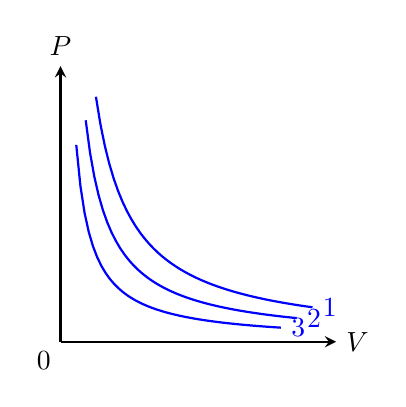
\begin{tikzpicture}[>=stealth, scale=1]
    % Koordinata o'qlari
    \draw[->, thick] (0,0) -- (3.5,0) node[right] {$V$};
    \draw[->, thick] (0,0) -- (0,3.5) node[above] {$P$};
    \node[below left] at (0,0) {0};

    % Izotermalarni chizish (P = k/V funksiyasi bo'yicha)
    % 1-izoterma (eng yuqori harorat)
    \draw[blue,thick, domain=0.45:3.2, samples=50] plot (\x, {1.4/\x}) node[right] {1};
    
    % 2-izoterma (o'rta harorat)
    \draw[blue,thick, domain=0.32:3.0, samples=50] plot (\x, {0.9/\x}) node[right] {2};
    
    % 3-izoterma (eng past harorat)
    \draw[blue,thick, domain=0.2:2.8, samples=50] plot (\x, {0.5/\x}) node[right] {3};

\end{tikzpicture}

\begin{enumerate}[label=\Alph*)]
\item 1
\item 3
\item 2
\item barchasi bir xil
\end{enumerate}

\item $V_1 = 10 \, l$ hajmli ballonni 100 kPa bosimda havo qamalgan. $30 \, l$ hajmli ballon bilan tutashtirilganda umumiy bosim 200 kPa ga teng bo‘lishi uchun $V_2$ hajmli ballonga qanday bosimda havo qamash lozim (kPa)?
\begin{enumerate}[label=\Alph*)]
\item 250
\item 275
\item 200
\item 233,3
\end{enumerate}

\item Hajmlari 3 l va 2 l bo‘lgan va kranli nay yordamida bir-biri bilan tutashtirilgan ikki idish turli gazlar bilan mos ravishda 20 kPa va 40 kPa bosim ostida to‘ldirilgan. Kran ochilgach temperatura o‘zgarmasa idishlarda qanday (kPa) bosim qaror topadi?
\begin{enumerate}[label=\Alph*)]
\item 28
\item 12
\item 16
\item 14
\end{enumerate}

\item 40 l va 20 l hajmli ikki idishda temperaturasi bir xil, lekin bosimi har xil gaz bor. Idishlar tutashtirilgandan keyin ularda 1 MPa bosim qaror topdi. Agar kichik idishdagi boshlang‘ich bosim 600 kPa bo‘lsa, katta idishdagi boshlang‘ich bosim qancha bo‘lgan (MPa)?
\begin{enumerate}[label=\Alph*)]
\item 2,6
\item 1,2
\item 1,8
\item 3,6
\end{enumerate}

\item Ikki uchi berk gorizontal silindr porshen bilan uch seksiyaga bo‘lingan. Har bir seksiyaning bosimi va hajmi mos ravishda $2 \cdot 10^4$ Pa va $36 \, sm^3$, $6 \cdot 10^4$ Pa va $60 \, sm^3$, $5 \cdot 10^4$ Pa va $104 \, sm^3$. Ikkinchi seksiyadagi gazning porshenlar bo‘shatilgandan keyingi bosimi (Pa) va hajmini aniqlang ($sm^3$).
\begin{enumerate}[label=\Alph*)]
\item $8 \cdot 10^4$; 45
\item $4 \cdot 10^4$; 45
\item $4 \cdot 10^4$; 4,5
\item $2 \cdot 10^4$; 25
\end{enumerate}

\item Germetik, uzunligi 1 metr bo‘lgan silindr ishqalanishsiz harakatlana oladigan porshen bilan teng ikkiga bo‘lingan. Bir tomondagi bosim ikkinchisidan ikki marta katta bo‘lsa, porshen bo‘shatilganda qanday masofaga siljiydi (m)?
\begin{enumerate}[label=\Alph*)]
\item 0,4
\item 0,2
\item 0,33
\item 1/6
\end{enumerate}

\item Ko‘lning tubidagi havo pufagi suv yuziga chiqquncha 4 marta kattalashadi. Havzaning chuqurligi qanday (m)? $T = const$.
\begin{enumerate}[label=\Alph*)]
\item 25
\item 30
\item 15
\item 10
\end{enumerate}

\item 20 m chuqurlikdagi ko‘lning tubidan havo pufakchasi suv sirtiga ko‘tarilganda, uning hajmi necha marta ortadi?
\begin{enumerate}[label=\Alph*)]
\item 2
\item 3
\item 7
\item 10
\end{enumerate}

\item Hovuz tubida hosil bo‘lgan gazli pufakcha diametri suv sirtiga yetganida 1,1 marta ortgan. Hovuzning chuqurligini (m) toping.
\begin{enumerate}[label=\Alph*)]
\item 1
\item 2
\item 3,3
\item 4
\end{enumerate}

\item 5 m chuqurlikdagi suvda suzib yurgan havo pufakchasining hajmi $5 \, mm^3$ ga teng. Suv yuziga qalqib chiqqan havo pufakchasining hajmi qanday bo‘ladi ($mm^3$)?
\begin{enumerate}[label=\Alph*)]
\item 5,3
\item 6
\item 6,5
\item 7,1
\end{enumerate}

\item Hovuz tubida hosil bo‘lgan pufakcha diametri suv sirtiga yetganida 1,2 marta oshgan. Hovuzning chuqurligini (m) toping.
\begin{enumerate}[label=\Alph*)]
\item 6,68
\item 5,48
\item 6,24
\item 7,28
\end{enumerate}

\item Hajmi 12 l bo‘lgan avtomobil kamerasidagi bosim 35 atm ga teng bo‘lishi kerak. Har bir dam berishda normal bosimda $500 \, sm^3$ havo oladigan nasos bilan necha marta dam berish kerak bo‘ladi?
\begin{enumerate}[label=\Alph*)]
\item 120
\item 168
\item 840
\item 420
\end{enumerate}

\item Boyl-Mariot qonunini tekshirish uchun mo‘ljallangan naychada uzunligi 75 mm bo‘lgan simob ustuni bor. Naycha yopiq uchi pastga qaratilgan holda vertikal qo‘yilganda havo ustunining uzunligi 120 mm, naycha gorizontal qo‘yilganda esa 132 mm bo‘lgan. Atmosfera bosimini aniqlang (Pa).
\begin{enumerate}[label=\Alph*)]
\item $2,0 \cdot 10^5$
\item $1,0 \cdot 10^2$
\item $1,0 \cdot 10^5$
\item $1,0 \cdot 10^4$
\end{enumerate}

\item Hajmi 12 l bo‘lgan avtomobil kamerasidagi bosim 35 atm ga teng bo‘lishi kerak. Agar kamera dastlabki holatda bo‘sh bo‘lsa (1 atm), har bir dam berishda $500 \, sm^3$ havo oladigan nasos bilan necha marta dam berish kerak bo‘ladi?
\begin{enumerate}[label=\Alph*)]
\item 816
\item 470
\item 340
\item 940
\end{enumerate}

\item Porshenli nasos bilan 2 l hajmli ballondan havosi so‘rib olinmoqda. Porshenning har bir yurishida ballondagi bosim 1,2 marta kamayadi. Nasos so‘rish kamerasining hajmini aniqlang (l).
\begin{enumerate}[label=\Alph*)]
\item 0,16
\item 1,2
\item 0,2
\item 0,4
\end{enumerate}

\item Agar porshenli nasosning har bir harakatida bosim 1,2 marta kamaysa, 4 l hajmli ballondan havoni so‘rib olish uchun nasosning kamerasining hajmi qanday bo‘lishi kerak (l)?
\begin{enumerate}[label=\Alph*)]
\item 8
\item 0,8
\item 0,2
\item 2
\end{enumerate}

\item Vertikal o‘rnatilgan ostki uchi kavsharlangan shisha nayning ichida geliy gazi va gazning ustida qalinligi 6 sm bo‘lgan simob ustuni bor. Nayning ochiq uchi pastga qaratib to‘nkarilganda, undagi simob ustunining qalinligi 5 sm bo‘lib qoldi. Nayning uzunligini toping (sm). $T = const$.
\begin{enumerate}[label=\Alph*)]
\item 14,4
\item 17,4
\item 8,7
\item 6,45
\end{enumerate}

\item Vertikal o‘rnatilgan ostki uchi kavsharlangan shisha nayning ichida geliy gazi va ustida 2 sm bo‘lgan simob ustuni bor. Nayning ochiq uchi pastga qarab to‘nkarilganda undagi simob ustining qalinligi 1 sm bo‘lib qoldi. Nayning uzunligini toping (sm).
\begin{enumerate}[label=\Alph*)]
\item 39,5
\item 32
\item 36,8
\item 27
\end{enumerate}

\end{enumerate}



\begin{table}[h!]
\centering
\begin{tabular}{|c|c|c|c|c|c|c|c|c|c|}
\hline
№ & J. & № & J. & № & J. & № & J. & № & J. \\ \hline
1 & D & 7 & C & 13 & D & 19 & B & 25 & A \\ \hline
2 & B & 8 & B & 14 & A & 20 & C & 26 & D \\ \hline
3 & D & 9 & A & 15 & C & 21 & C & 27 & B \\ \hline
4 & C & 10 & D & 16 & A & 22 & D & 28 & D \\ \hline
5 & A & 11 & A & 17 & D & 23 & C & 29 & D \\ \hline
6 & D & 12 & A & 18 & B & 24 & C & & \\ \hline
\end{tabular}
\end{table}